\PassOptionsToPackage{unicode=true}{hyperref} % options for packages loaded elsewhere
\PassOptionsToPackage{hyphens}{url}
%
\documentclass[12pt,]{article}
\usepackage{lmodern}
\usepackage{amssymb,amsmath}
\usepackage{ifxetex,ifluatex}
\usepackage{fixltx2e} % provides \textsubscript
\ifnum 0\ifxetex 1\fi\ifluatex 1\fi=0 % if pdftex
  \usepackage[T1]{fontenc}
  \usepackage[utf8]{inputenc}
  \usepackage{textcomp} % provides euro and other symbols
\else % if luatex or xelatex
  \usepackage{unicode-math}
  \defaultfontfeatures{Ligatures=TeX,Scale=MatchLowercase}
\fi
% use upquote if available, for straight quotes in verbatim environments
\IfFileExists{upquote.sty}{\usepackage{upquote}}{}
% use microtype if available
\IfFileExists{microtype.sty}{%
\usepackage[]{microtype}
\UseMicrotypeSet[protrusion]{basicmath} % disable protrusion for tt fonts
}{}
\IfFileExists{parskip.sty}{%
\usepackage{parskip}
}{% else
\setlength{\parindent}{0pt}
\setlength{\parskip}{6pt plus 2pt minus 1pt}
}
\usepackage{hyperref}
\hypersetup{
            pdftitle={A Methodological Approach Comparison to Estimate Mortality in Small Areas: the Pampean Region in Argentina (2009-2011)},
            pdfborder={0 0 0},
            breaklinks=true}
\urlstyle{same}  % don't use monospace font for urls
\usepackage[margin=1in]{geometry}
\usepackage{graphicx,grffile}
\makeatletter
\def\maxwidth{\ifdim\Gin@nat@width>\linewidth\linewidth\else\Gin@nat@width\fi}
\def\maxheight{\ifdim\Gin@nat@height>\textheight\textheight\else\Gin@nat@height\fi}
\makeatother
% Scale images if necessary, so that they will not overflow the page
% margins by default, and it is still possible to overwrite the defaults
% using explicit options in \includegraphics[width, height, ...]{}
\setkeys{Gin}{width=\maxwidth,height=\maxheight,keepaspectratio}
\setlength{\emergencystretch}{3em}  % prevent overfull lines
\providecommand{\tightlist}{%
  \setlength{\itemsep}{0pt}\setlength{\parskip}{0pt}}
\setcounter{secnumdepth}{0}
% Redefines (sub)paragraphs to behave more like sections
\ifx\paragraph\undefined\else
\let\oldparagraph\paragraph
\renewcommand{\paragraph}[1]{\oldparagraph{#1}\mbox{}}
\fi
\ifx\subparagraph\undefined\else
\let\oldsubparagraph\subparagraph
\renewcommand{\subparagraph}[1]{\oldsubparagraph{#1}\mbox{}}
\fi

% set default figure placement to htbp
\makeatletter
\def\fps@figure{htbp}
\makeatother

\usepackage{booktabs}
\usepackage{longtable}
\usepackage{array}
\usepackage{multirow}
\usepackage{wrapfig}
\usepackage{float}
\usepackage{colortbl}
\usepackage{pdflscape}
\usepackage{tabu}
\usepackage{threeparttable}
\usepackage{threeparttablex}
\usepackage[normalem]{ulem}
\usepackage{makecell}
\usepackage{xcolor}

\title{A Methodological Approach Comparison to Estimate Mortality in Small
Areas: the Pampean Region in Argentina (2009-2011)}
\author{Nicolás Sacco;\footnote{Penn State,
  \href{mailto:nsacco@psu.edu}{\nolinkurl{nsacco@psu.edu}}} Iván
Williams;\footnote{Universidad Nacional de Luján,
  \href{mailto:ivanwilliams1985@gmail.com}{\nolinkurl{ivanwilliams1985@gmail.com}}}
Bernardo L. Queiroz\footnote{Cedeplar-UFMG,
  \href{mailto:lanza@cedeplar.ufmg.br}{\nolinkurl{lanza@cedeplar.ufmg.br}}}}
\date{Aug, 2019}

\begin{document}
\maketitle

\hypertarget{abstract}{%
\section{\texorpdfstring{\textbf{Abstract}}{Abstract}}\label{abstract}}

\hypertarget{background}{%
\subsection{\texorpdfstring{\textbf{Background}}{Background}}\label{background}}

While the demand for epidemiological estimates of small areas is
growing, recent studies show a wide gap and persistent inequalities in
life expectancy at birth in Latin America. The lack of geospatial data
challenge the application of different methods to study health
differentials. Often data in small areas are non-existent or sparce in
this region. Spatial patterns are essential to understand individual
demographic outcomes related with the characteristics of a place, also
as a tool for the application of development plans and for the
allocation of resources.

\hypertarget{objectives}{%
\subsection{\texorpdfstring{\textbf{Objectives}}{Objectives}}\label{objectives}}

The history of estimation in small areas is scarce in Argentina, a clear
example of a country with few data sources, but also a very interesting
case of the epidemiological transition, often not address by the
previous literature. Based on the experience of new applications
according to the available auxiliary information, in this paper we apply
three different methods to estimate and then compare mortality levels in
small areas in the Pampean Region of Argentina, during the period
2009-2011.

\hypertarget{methods}{%
\subsection{\texorpdfstring{\textbf{Methods}}{Methods}}\label{methods}}

Life expectancy at birht was calculated based on a Bayesian approach, a
relational life-table method, smoothing spatial data `borrowing
strength' from neighboring areas, and third a indirect demographic
approach. Estimates are compared to calculate \(q_0\) rates from full
death registers and then related to spatial areas, using a simple
regionalization analysis.

\hypertarget{results}{%
\subsection{\texorpdfstring{\textbf{Results}}{Results}}\label{results}}

Results display the potential value of the Bayesian method at the small
area-spatial scale. Estimated rates indicate that there is a huge
variability in life expectancy at birht withing and between regions,
with a spread of up to more than 6 years in the Province of Buenos
Aires. Furthermore, we find suggestive evidence that the rates by age
present a higher infant mortality but also a higher risk in older
adults, in provinces that exibhit more heterogeneity.

\begin{center}\rule{0.5\linewidth}{0.5pt}\end{center}

\hypertarget{data}{%
\subsection{\texorpdfstring{\textbf{Data}}{Data}}\label{data}}

Death micro data for register years 2009, 2010 and 2011 was requested to
the Department of Health Statistics and Information (DEIS, acronym in
Spanish) of the Ministry of Health of the Nation. The late registration
in all the country was about 1.05\%, and the usual thought of
compensation is not uniform between years and small areas, so we decided
to process the database and take the registers by occurrence year
(\ref{tab:def_tardias}). The percentage of unknown age was 0.33\% and
unknown sex 1.01\%. The unknown department information by province is
ranked in \ref{tab:SinDEP}, being Ciudad Autónoma de Buenos Aires the
province in worst position. This 71\% is due to deaths that occurred in
adjacent or very close departments to CABA, in the Great Buenos Aires
(agglomerate in Buenos Aires province that is CABA's neighbor): Tres de
Febrero (20\%), Vicente Lopez (15\%), La Matanza (12\%), Avellaneda
(7\%), Lanús (5\%), Morón (5\%), San Isidro (4\%) y Gral. San Martín
(3\%).\footnote{Camisa (\protect\hyperlink{ref-Camisa_2019}{2019}) noted
  this bias a lot of years ago: 10\% of births and deaths during the
  period 1946-1948.} Also because of the change in the definition of the
administrative units in CABA, starting in 2011 in the data base, is not
possible to match the three risk years; because of both reasons was
decided leaving out of this first estimation.

The unknown data within small areas is an important issue
(\ref{tab:UnkSexAge}). Looking only the Pampean provinces, Buenos Aires
had the departments with highest percent of unknown age and sex, with
larger values in sex, being the leader the department General Pueyrredón
with 7.3\%. For that reason, in this first study we won't disagree the
estimation by sex. The unknown categories (in variables age, residence
province and residence department) were distributed proportionally.

For the exposure population for each department was used the estimated
population by INDEC at middle year in 2010, and applied the census
structure (INDEC (\protect\hyperlink{ref-INDEC2015}{2015})). Then,
instead of simple averaging the three death years, was taken in account
the year-person lived in the three year time window between 2009 and
2011 and the estimation date (Gonzaga and Schmertmann
(\protect\hyperlink{ref-Gonzaga_Schmertmann_2016}{2016})). This
procedure allowed, first to smooth a bit the age-heaping, that could be
a greater bias for rate comparison when the deaths count doesn't follow
this pattern by age; and second taking in advantage of the omission
corrections made by INDEC.\footnote{It's not clear the methodology
  applied for the adjusted population at middle year on departments, and
  if takes in account a ``residence'' correction (INDEC
  (\protect\hyperlink{ref-INDEC2015}{2015}))} For that was assume a
uniform distribution of birth date within a year and closed population.
A unique survival function was used for all the districts, applying the
same standard life tables than the authors (a representative mean of the
Human Mortality Database in posterior years to 1969) but weighted by a
male ratio of 1.04 at birth to get both sex. A similar smooth, but with
less demographic interpretation, can be achieved with local regression
on 3 times the population count (James et al.
(\protect\hyperlink{ref-James2014}{2014})) (see \ref{fig:AdjExp}).

\begin{figure}

{\centering 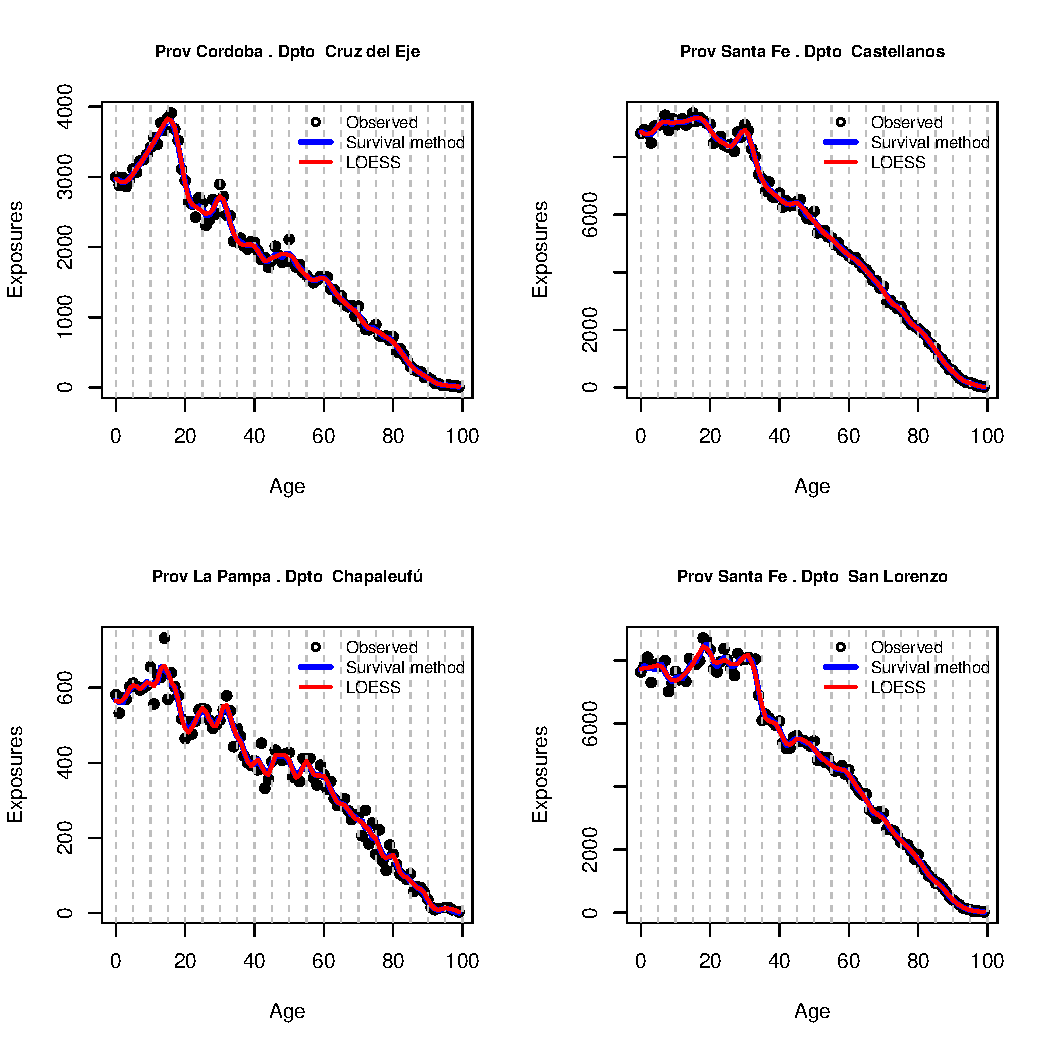
\includegraphics[width=0.7\linewidth]{analysis/plots/AdjExp} 

}

\caption{Exposure Adjustment 2008-2010. Four cases. Source: own based in Census}\label{fig:AdjExp}
\end{figure}

\hypertarget{some-consistency-cheks}{%
\subsection{\texorpdfstring{\textbf{Some consistency
cheks}}{Some consistency cheks}}\label{some-consistency-cheks}}

There are increasing attempts to address the death coverage problem,
depending on the auxiliary information that is counted (Preston et al.
(\protect\hyperlink{ref-Preston1980}{1980}); Bennett and Horiuchi
(\protect\hyperlink{ref-Bennett_Horiuchi_1984}{1984}); Schmertmann and
Gonzaga (\protect\hyperlink{ref-Schmertmann2018}{2018})). The
utilization of demographic indirect methods of coverage evaluation are
difficult to maintain in small population very influenced by internal
migration and low exposures.

With the aim to visualize possible problems of quality data in
departments, two consistency checks were performed.

First, we calculated the \(P/F\) method for indirect estimation of
infant mortality and mapped against \(q_0\) from the raw data obtained
in the last section (Moultrie et al.
(\protect\hyperlink{ref-Moultrie}{2013})). This is not an accurate
method for small populations, but can give an idea about problems in
biggest areas (numerator or denominator rates). We show the unweighted
and weighted points to give more importance to consistency in populated
areas, who was responsible for the smoothness bias in the methodological
procedures described in next section. Using the mean age at birth for
each province and the Latin America family of UN tables for the
estimation, looking infant mortality points there is no obvious bias in
the biggest areas, and no reason for exclude them (\ref{fig:PF}).

\begin{figure}

{\centering 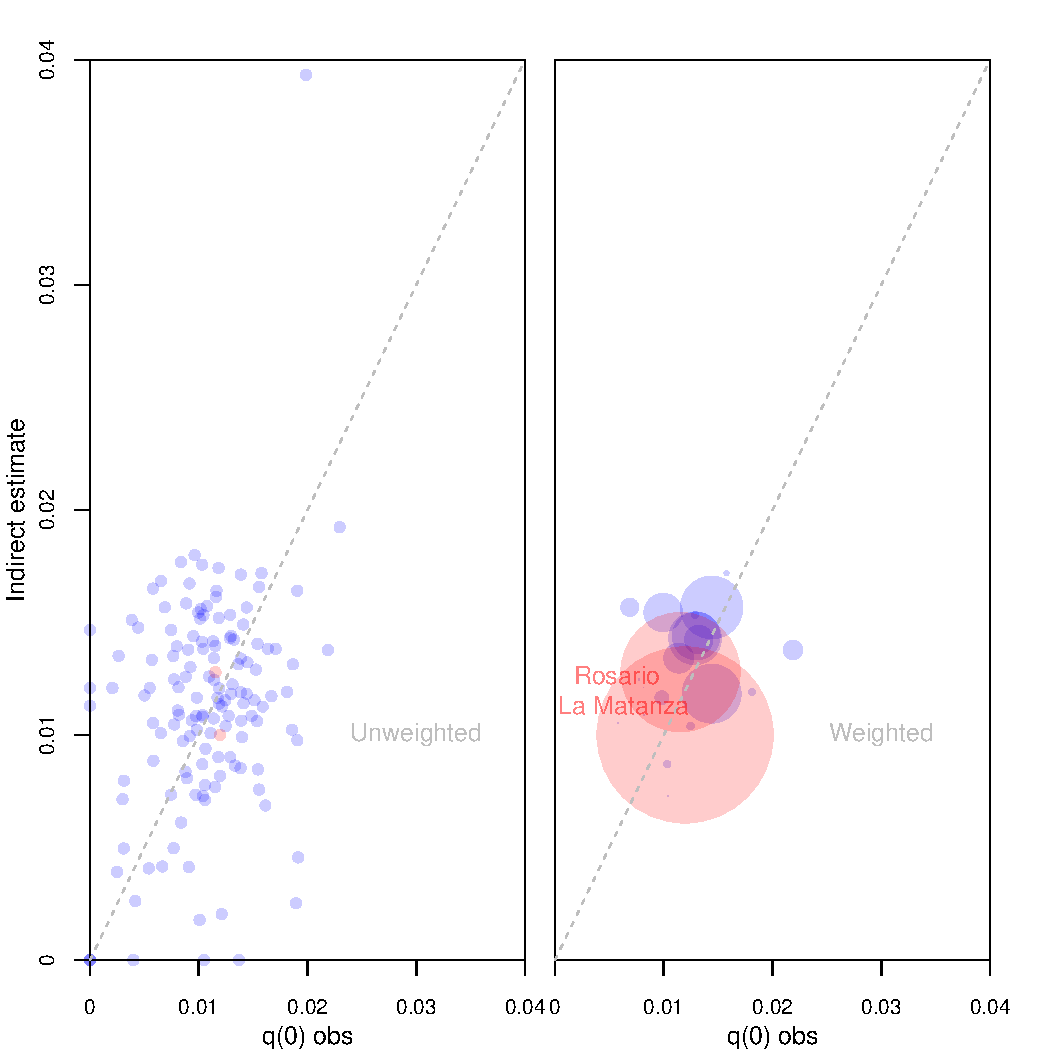
\includegraphics[width=0.7\linewidth]{analysis/plots/ChekPF} 

}

\caption{Indirect estimates and raw infant mortality. Departments in selected provinces. Source: own based in Census and DEIS}\label{fig:PF}
\end{figure}

Second, was mapped each department against the census poverty indicator
Unsatisfied Basic Needs (NBI in Spanish, that will be introduced after),
looking for some expected relationship (Kaztman
(\protect\hyperlink{ref-Kaztman1995}{1995}), Preston
(\protect\hyperlink{ref-Preston_1975}{1975}); Grushka
(\protect\hyperlink{ref-Grushka2013}{2013})). In \ref{fig:NBI} are
showed the NBI3 and NBI4, which measures the percentaje of school
absence of children and substense incapacity in housing units (Kaztman
(\protect\hyperlink{ref-Kaztman1995}{1995})). In color is highlighted
the biggest department in the Pampean Region, called La Matanza (having
10.7398421\% of the province Buenos Aires). La Matanza department has
one of the lowest standardized mortality rate, but similar poverty index
than others. Looking its performance in the poverty indexes 1 (poor
housing), 2 (toilet available) and 3 (average persons by house), and
having the lowest standardized mortality rate (using all region
structure), it was decided to leave it out this study, where the biggest
areas has the importance to smooth the small ones and this could bias
the results. This correction is already advised in the INDEC warning of
department population counts in 2010 Census, where Buenos Aires is one
of the provinces with coverage issues.\footnote{(\url{https://www.indec.gob.ar/nivel4_default.asp?id_tema_1=2\&id_tema_2=24\&id_tema_3=119},
  visited on 25/2/19}

\begin{figure}

{\centering 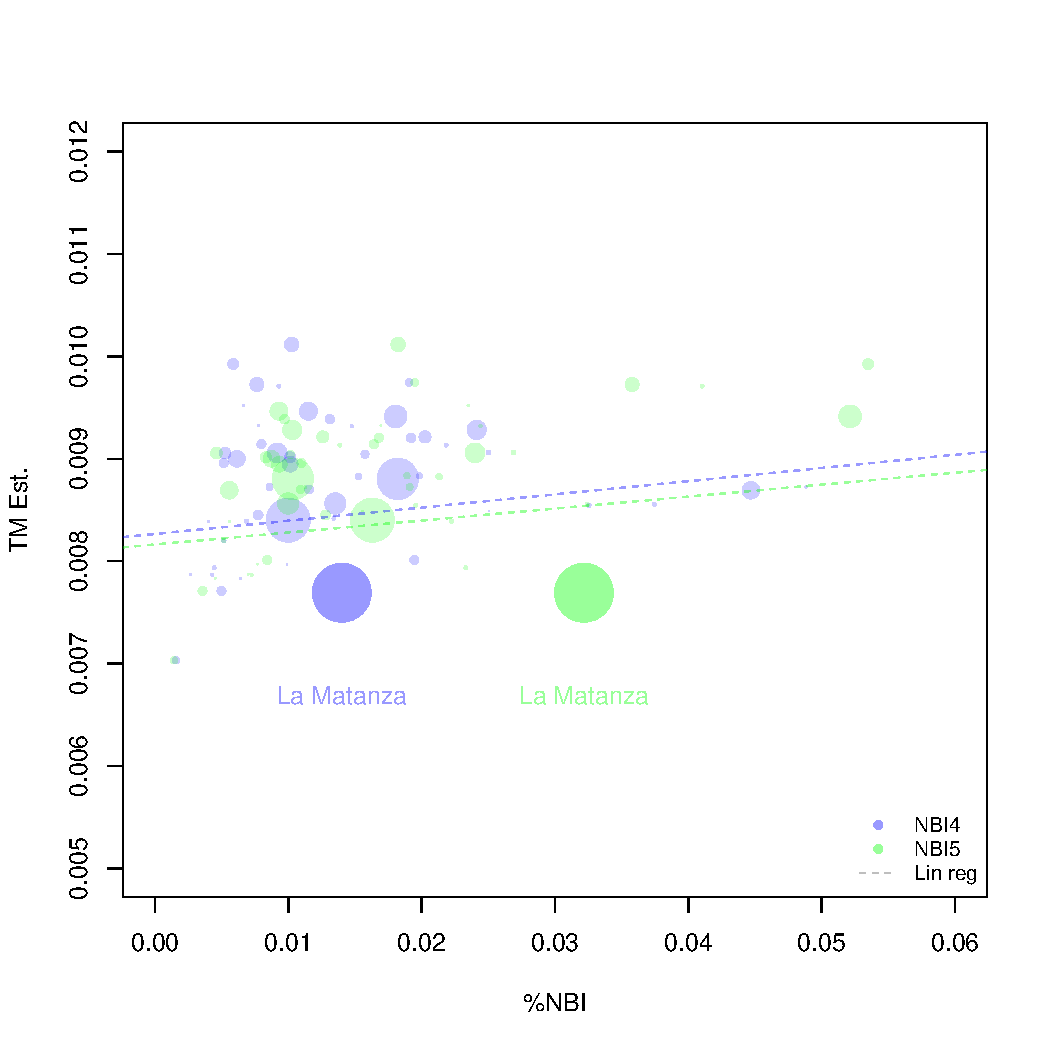
\includegraphics[width=0.7\linewidth]{analysis/plots/ChekNBI} 

}

\caption{Standarized mortality rate and NBI. Departments in selected provinces. Source: own based in Census and DEIS}\label{fig:NBI}
\end{figure}

An additional check was calculate the \(e_0\) for each province using
the inputs described before and the INDEC estimation (INDEC
(\protect\hyperlink{ref-INDEC2013}{2013})). The results are a relative
difference (\%) of 0, 0.39, 0.3, 0.98, 0.34 for provinces Buenos Aires,
Cordoba, Entre Rios, La Pampa, Santa Fe, considered an acceptable
approximation given the one year of distance in temporal reference
(\ref{tab:Dif_e0_INDEC}).

\hypertarget{methodology}{%
\subsection{\texorpdfstring{\textbf{Methodology}}{Methodology}}\label{methodology}}

Due to the fact that is the first estimation in departments in Argentina
(at least that is known by the authors), was decided to apply three
techniques: one based in Bayesian theory, the second one based in
relational life-table methods but adding statistical smoothing, and
third a classical demographic approach that is considered the default
method. Before the estimation, a regionalization procedure was done to
take advantage of spatial similitude between small areas.

\hypertarget{regionalization}{%
\subsubsection{\texorpdfstring{\textbf{Regionalization}}{Regionalization}}\label{regionalization}}

The definition of a region or cluster must exploit the internal
similarity between small areas to be able to suppose that their
mortality are realizations of a greater stochastic process. The
similarity in mortality patterns use to be approached because of
belonging to the same province, where the ``distance'' between
jurisdictions is not measured by geographical distance or socio-economic
attributes (Data and Estimation
(\protect\hyperlink{ref-Longford2005}{2019})).

To consider this we take the approach given by Assuncao et al.
(\protect\hyperlink{ref-AssunCao2006}{2006}), which tried to define
larger areas internally homogeneous and with contiguous regions in
space. First is done a connectivity graph between centroids and then is
calculated the cost between them (euclidean distance in our case). Then,
an iteration procedure estimates the minimum spanning tree, which is the
connected tree with minimum cost, measured as the sum of the
dissimilarities over all the edges. Finally, a partition procedure is
made cutting the edge that minimize the variance within the resulting
two clusters. Because testing all the possible combinations at each
partition is a computational problem, the authors proposed an heuristic
approach. An overclusterization would increase homogeneity but also
increase variance in smallest units because of not enough exposures.
That´s the reason because of a population threshold must be settled.

As inputs for the regionalization procedure we use the shape files
available online\footnote{\url{https://redatam.indec.gob.ar/} , visited
  on 25/2/19.} and the census index Unsatisfied Basic Needs (NBI in
Spanish), both by department, available in INDEC webpage.\footnote{Same
  date.} We scaled the index to standard deviation units and applied the
methodology of commented before, implemented in the \emph{spdep}
package, with the function \emph{skater} (Bivand
(\protect\hyperlink{ref-Bivand2019}{2019})).

With this segmentation was obtained an increase of 14\% in the variance
between groups and a decrease of 1\% in the average variance within each
group. The new cluster is more distinct between them, and with less
internal relative variance (see \ref{fig:cluster}). We'll use this
grouping for the calculations of two of the next three methods applied.

\begin{figure}

{\centering 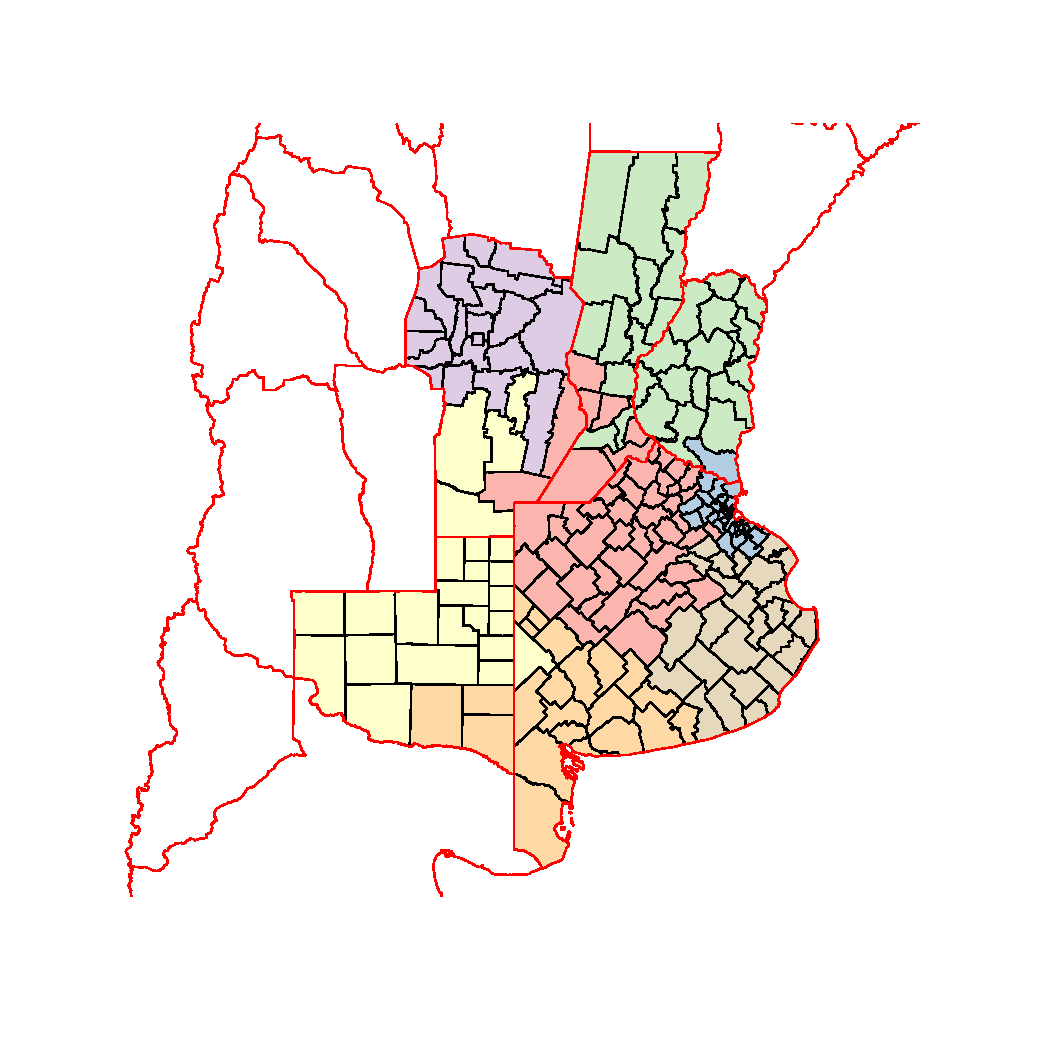
\includegraphics[width=0.7\linewidth]{analysis/plots/cluster} 

}

\caption{Regionalization of departments. Source: own based in Census and DEIS}\label{fig:cluster}
\end{figure}

\hypertarget{estimation-methods}{%
\subsubsection{\texorpdfstring{\textbf{Estimation
Methods}}{Estimation Methods}}\label{estimation-methods}}

Although Argentina is usually classified as a country with good death
statistics (Jaspers and Orellana
(\protect\hyperlink{ref-JaspersOrellana1994}{1994})), from what is known
there is an unequal percentage of child deaths not registered by
province years ago (DEIS (\protect\hyperlink{ref-DEIS2016}{2016})). In
this sense, since the source of data is a registry, thinking about the
estimation of mortality rates by age, one might think that there is no
variance, and the bias (both components of the mean squared error of an
estimator) would be given by the pattern of cases omitted in each
jurisdiction. As was mentioned before, the second component of the error
will not be addressed in this work because of no information about its
distribution by small areas (and is mentioned as a the main limitation
in next sections). Regarding the first, there are phenomena with a small
number of ``experiments'' (few exposed in our case), which have a
greater variance in their estimates, so it requires special treatment in
order to reflect the risk of underlying mortality (Brillinger
(\protect\hyperlink{ref-Brillinger1986}{1986})). For achieving that we
will use and compare three different methods, which have in common that
take advantages of the information in the grater area.

The Empirical Bayesian method improves the statistical efficiency of the
estimators of mortality rates by age, decreasing the variance in the
cases of small jurisdictions (Efron and Morris
(\protect\hyperlink{ref-Efron1972}{1972}); Marshall
(\protect\hyperlink{ref-Marshall1991}{1991}); Data and Estimation
(\protect\hyperlink{ref-Longford2005}{2019}); Assunção et al.
(\protect\hyperlink{ref-Assuncao2005}{2005})). The idea is that assuming
that the different observations of each area proceeds from a common
prior, each estimation can be improved using information from the other
ones. The prior distribution corresponds to the joint distribution of
the vector of mortality rates by age of the largest area. Then, through
the observed behavior in each minor area, the Bayesian adjustment of the
posterior mortality distribution occurs. The characteristic of
``empiric'' is that the distributions of the parameters of the greater
area are estimated, in this case by the method of moments, also from the
data.

Let's see first the univariable case. Considering a five-year age group
either in an area \(i\), the distribution of deaths \(d\) is assumed to
be a Poisson process, with expected mean
\(E(d_{x, 4} ^ {i}|{m_{x,4}^{i} }) = N_{x, 4}^{i} m_{x, 4}^{i}\), being
\(N\) the exposures and \(m\) the mortality rate.

First consider \(\hat{m}_{x,4}^{i} = D_{x,4}^{i}/N_{x,4}^{i}\) as the
maximum likelihood estimator of the rate \(m_{x,4}^{i}\) in the area
\(i\), which are \(iid\) generated from \(m_{x,4}\). The conditioned
expectancy of \(\hat{m}_{x,4}^{i}\) is
\(E_{m}(E({\hat{m}}_{x,4}^{i})/m_{x,4}^{i})=E_{m}({m_{x,4}^{i}})=m_{x,4}\)
(big area rate), and conditioned variance
\(V({\hat{m}}_{x,4}^{i}/m_{x,4}^{i}) = \frac{m_{x,4}^{i}}{N_{x,4}^{i}}\).

The total variance of the estimator can be expressed as the sum of the
variance of the \(i's\) means and the expectancy of the \(i's\)
variances:
\(V_{m}(E(\hat{m}_{x,4}^{i}/m_{x,4}^{i})) + E_{m}(V({\hat{m}}_{x,4}^{i}/m_{x,4}^{i}))= V_{m}(\hat{m}_{x,4}^{i}) + E_{m}(\frac{{\hat{m}}}{N_{x,4}^{i}}) = V_{m}(m_{x,4}^{i}) + \frac{m_{x,4}}{N_{x,4}^{i}}\).
That is related to the hierarchical relation between the hyper parameter
(\(m_{x,4}\)), the parameters (\(m_{x,4}^{i}\)) and its estimators
\(\hat{m}_{x,4}^{i}\).

The Bayesian linear estimator \(\mathring{m}_{x, 4}^{i}\) which
minimizes the mean squared error of \({m}_{x,4}^{i}\) (and indicators
that are linear functions of this) is (Robbins, 1983):

\(\mathring{m}_{x,4}^{i}=\hat{m}_{x,4}^{i}+S_{x,4}^{i}(\bar{m}_{x,4}^{i}-\hat{m}_{x,4}^{i})\)

Again, it is empirical because \(m_{x,4}\) is estimated by method of
moments with \(\bar{m}_{x,4}\), the weighted mean of small areas. The
``shrinkage'' factor \(S_{x,4}^{i}\) is the ratio between the expectancy
of the estimated variance in the small area \(i\) and the unconditioned
variance of the estimator, which is:

\(S_{x,4}^{i}=\frac{V_{m}(m_{x,4}^{i})}{V_{m}(m_{x,4}^{i})+\frac{m_{x,4}}{N_{x,4}^{i}}}\)

Or seen in another way, this formula represents the ratio between the
variance of the smaller area with respect to the sum of the total
variance (of the smaller and larger area), in tune with an analysis of
the classic variance between groups (ANOVA). Following this reasoning,
in a context of extreme homogeneity, a very small minor area could be
characterized from the estimation of the largest area
(\(S_{x,4}^{i}\cong 1\)). On the other hand, areas of high population
weight will take values close to those observed
(\(S_{x,4}^{i}\cong 0\)). In the middle of these extremes, the function
linearly combines the estimate of the big area with respect to the
smallest area included.

Longford (\protect\hyperlink{ref-Longford1999}{1999}) extended this idea
to vectors of random variables from smaller areas (``multivariate
shrinkage''), estimating \(S_{x,4}^{i}\) taking advantage of the
correlation between sub-populations across areas. In our case, if the
mortality rate of the age group between \(x\) and \(x + 4\) of area
\(i\) is greater than area \(j\), a high correlation would imply that in
a contiguous ages the same would happens with more chance. If covariance
were null, this approach would be equivalent to univariate case
described before. The calculations done in this work were done for ages
0, 1-4, and quinquennial ages until the open aged group 80. The
development was done following the approach showed in Assunção et al.
(\protect\hyperlink{ref-Assuncao2005}{2005}) (pages 543 and 544), which
estimated the parameters by the method of moments for fertility rates in
Brazil.

The other method that will be applied is based in a relational mortality
model called TOPALS (Tool for Projecting Age-Specific rates using Linear
Splines) (Beer (\protect\hyperlink{ref-deBeer2011}{2011})), which uses a
linear spline to describe the ratios between the age-specific death
probabilities of a given population and a standard age schedule. One
advantage against the classical Brass logit approach, is that TOPALS is
less sensitive by the choose of the standard. Gonzaga and Schmertmann
(\protect\hyperlink{ref-Gonzaga_Schmertmann_2016}{2016}) included the
spline fit into a Poisson regression of the rates, allowing confidence
intervals for the results that take in account variance for low exposure
reason.

The vector of mortality rates in the small area
\(m^{i}(\alpha)=m^{*}* \exp^{\alpha B_{x}}\) is a function of the spline
``nodes'' \(\alpha\), which are the ages at which will be valuated the
offset from the standard, being \(m^*\) the standard mortality rate
vector, and \(B_{x}\) is the B-spline matrix that multiplied by
\(\alpha\) gives the lineal offset between the log-rates.

The idea is suppose \(D_{x}\sim Poi(m_{x}N_{x})\) in each small area,
construct the likelihood function using the observed deaths and
exposures
\(\log (L(m_{x}N_{x}|D_{x}))=\sum_{\forall x}{\lbrack -m_{x}N_{x}+D_{x}\ln (m_{x})+D_{x}\ln (N_{x})-\ln (D_{x}!)\rbrack}\),
but expressing that in function of the parameter \(\alpha\), and adding
a penalization for distance from the standard and smoothing between
adjacent ages for smoothness. Using 6 nodes at ages 0, 1, 10, 20, 40, 70
and 100 like the authors, the final log-likelihood to maximize is:
\(Q(\alpha )=\sum_{\forall x}{\lbrack -m(\alpha )_{x}N_{x}+D_{x}\ln(m(\alpha )_{x})\rbrack }-\sum_{k=0}^{5}{(\alpha _{k}-\alpha _{k+1})^{2}}\).

Finally, as the basic method, will be applied the Indirect
Standardization method, maybe one of the first approaches to this
problem (Arriaga (\protect\hyperlink{ref-Arriaga2011}{2011})). It is
based in change only the level of the major area to replicate the deaths
of the minor area that is being estimated. Is the case where no
consideration about specific mortality shape of the minor area is made.

The Empirical Bayesian method is particularly appropriate in cases with
``small local samples, substantial regional variations, strong relations
between schedule components, and known spatial relationships'' (Assunção
et al. (\protect\hyperlink{ref-Assuncao2005}{2005})). In the case of
TOPALS regression, the application is more a smoothness technique than a
spatial-variability model, so less assumptions about relationships
between areas are needed.

\hypertarget{results-1}{%
\subsubsection{\texorpdfstring{\textbf{Results}}{Results}}\label{results-1}}

The estimates were made for five-aged groups in all departments in
Pampean Region (except La Matanza and those in CABA). The TOPALS methods
was thought and applied before to simple ages, but in this case because
of no correction for omission in small areas, it was decided not to
increase uncertainty so was applied also in quinquennial ages with knots
in ages 0, 5-9, 20-24, 40-44 and 60-64. Four examples are shown in next
graph, where the differences between methods starts to appear when the
exposures are smaller (see \ref{fig:Ajuste}).

\begin{figure}

{\centering 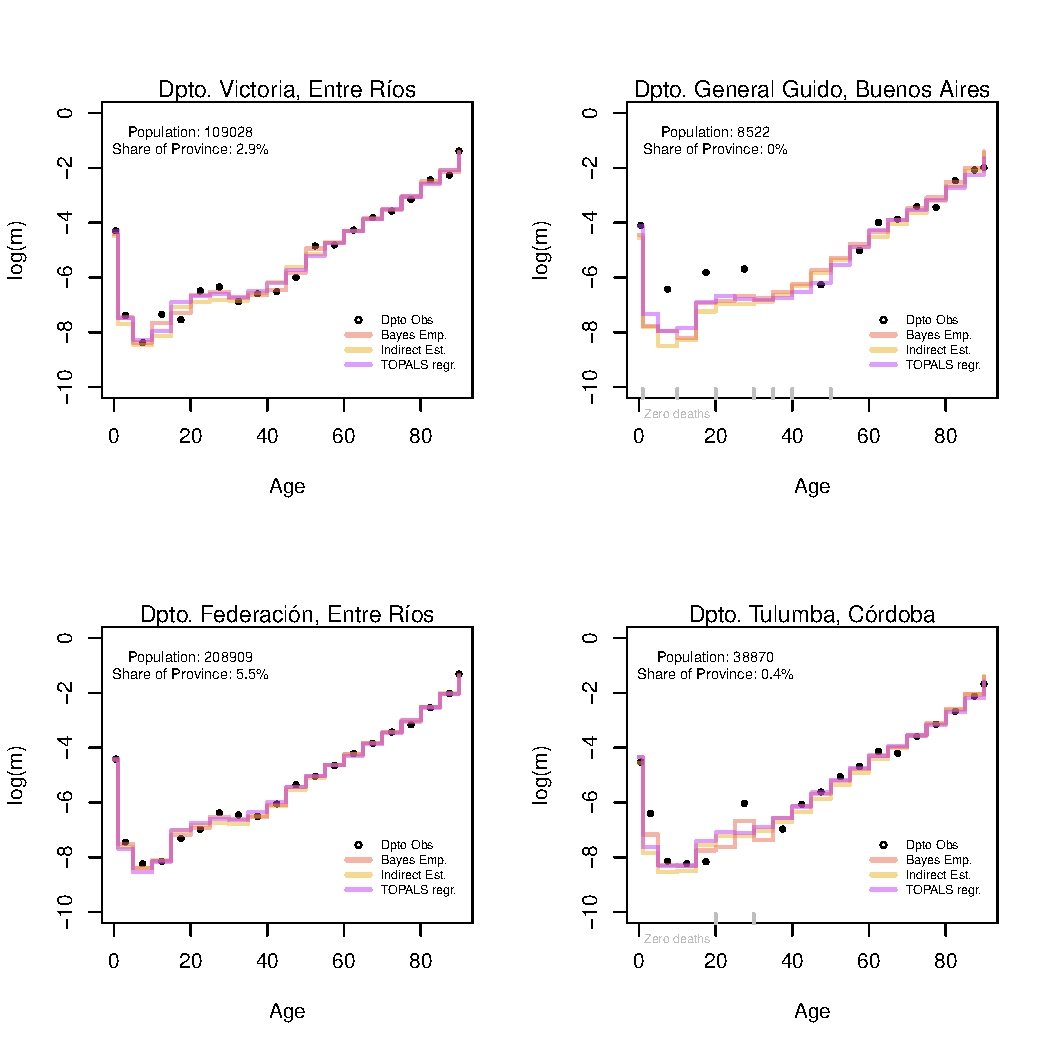
\includegraphics[width=0.7\linewidth]{analysis/plots/Ajuste} 

}

\caption{Mortality Estimates of Departments. Different methods. Source: own based in Census and DEIS}\label{fig:Ajuste}
\end{figure}

The \(e_0\) as the summary measure of mortality is considered to
compare, considering also that the effect of problems in adult ages
doesn´t affect hardly the estimates on \(e_0\) in populations where
infant, young and adult mortality still with an important
weight\footnote{In mathematical terms,
  \(\frac{de_0}{d\mu_{80+}}=f(T_{80+})\) are close to zero depending the
  non-rectangularity of \(l_x\) and the correction or change in the
  rate; in other therms a change in these rates, for example because of
  bias correction, is weighted by \(l_80\):
  \(\frac{de_0}{d\epsilon}=\int_{o}^{\inf}{\frac{d\mu_x}{d\epsilon}e_x l_x dx}\)
  (Wrycza and Baudisch (\protect\hyperlink{ref-Wrycza2012}{2012})).}

The correlation between the methods is clear: there is a strong
similitude between TOPALS and Indirect estimation (), but not so strong
in empirical Bayes against Indirect estimation (), and TOPALS () (see
\ref{fig:comparativeMeth}).

\begin{figure}

{\centering 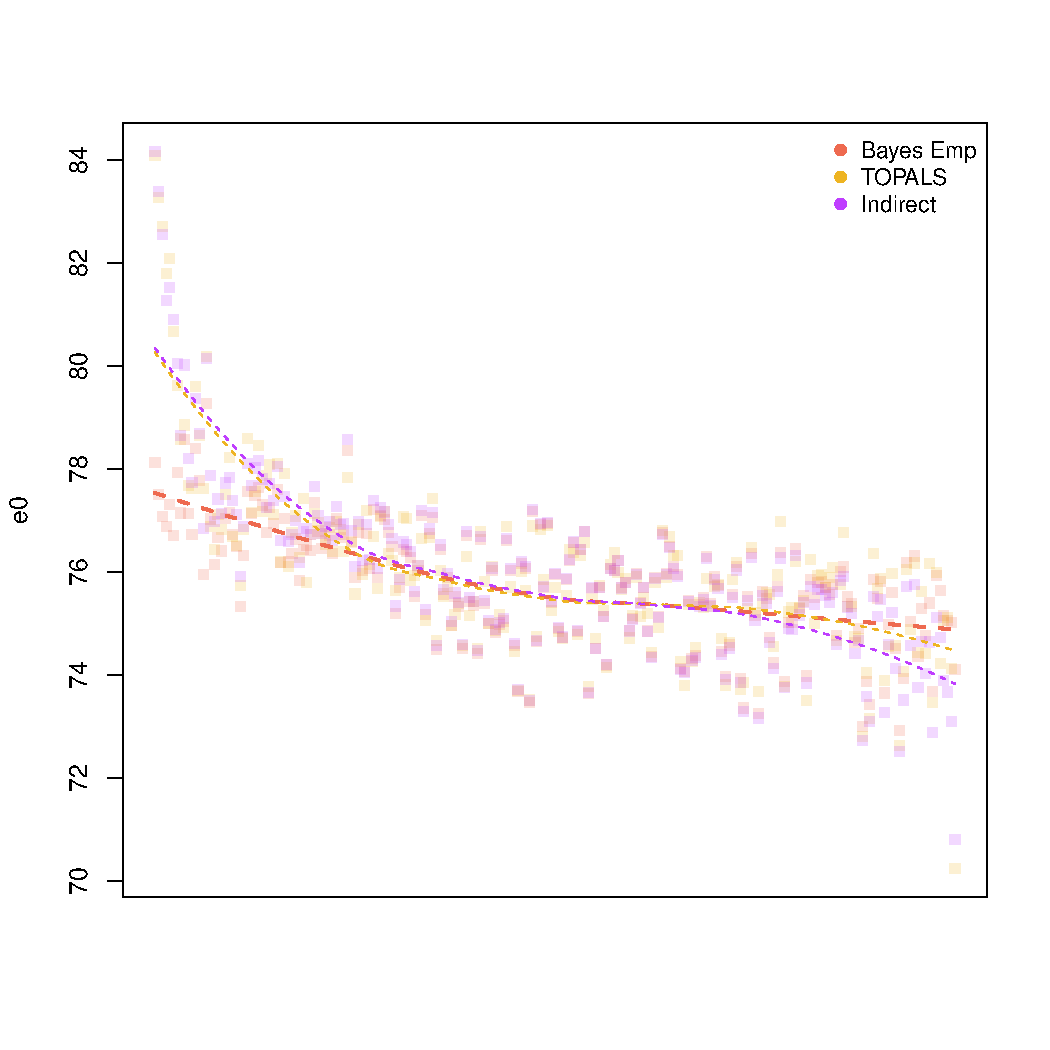
\includegraphics[width=0.7\linewidth]{analysis/plots/CompMethods} 

}

\caption{Estimates of life expectancy at birth with three methods. Source: own based in Census and DEIS}\label{fig:comparativeMeth}
\end{figure}

The main differences are because the Bayesian method tends to take
always some information about the age pattern, and assumes a correlation
between them. The departments with biggest differences are all of small
populations and few non-zero cells (see \ref{fig:Feos}).

\begin{figure}

{\centering 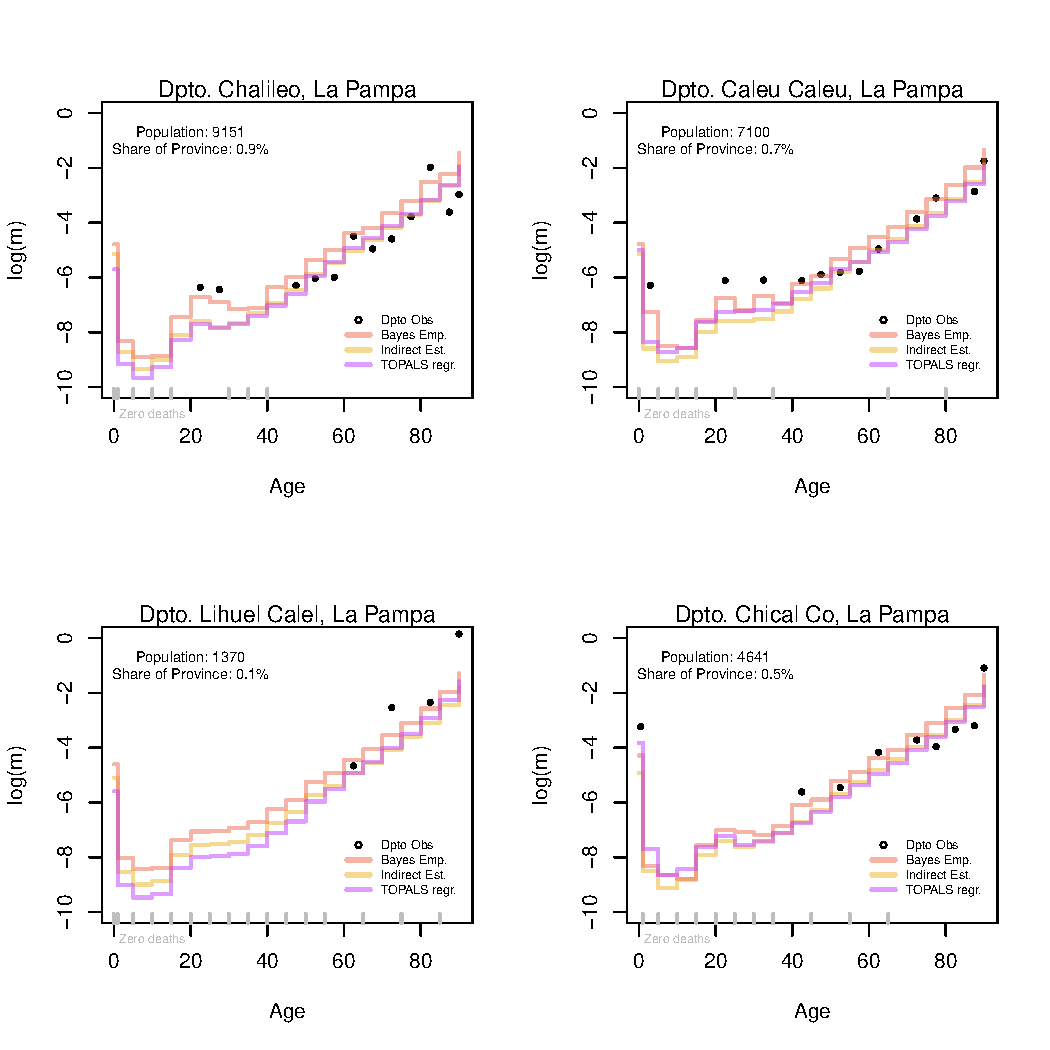
\includegraphics[width=0.7\linewidth]{analysis/plots/AjusteFeos} 

}

\caption{Mortality Estimates of Departments with largest differences between methods. Source: own based in Census and DEIS}\label{fig:Feos}
\end{figure}

In the next we'll take the Bayes empirical results because of the
conservative scenario in ranking departments.\footnote{A simulation
  study will be done here to achieve stronger conclusions} To take
randomness in account, bootstrap re-sampling of the death counts
following a Poisson distribution was done. This gave us confidence
intervals of the life table functions and specifically of life
expectancy at birth (see \ref{fig:jerarq} and \ref{tab:table_e0}).

\textbf{An analysis: Buenos Aires}

Buenos Aires is the most populous province in Argentina, including 134
administrative areas. In the previous graph was shown his great
heterogeneity, with an estimated range in life expectancy of
approximately 6 years. The province can be divided between the Great
Buenos Aires area made of 24 departments, an urban area that rounds
CABA, and the rest of the surface. To inspect the meaningful of the
results, we can take four jurisdictions with not small exposures and
placed along the distribution: San Isidro, Chivilcoy, General Pueyrredón
y Moreno (see \ref{fig:dptosBsAs}).

\begin{figure}

{\centering \includegraphics[width=0.7\linewidth]{analysis/plots/dptosBsAs} 

}

\caption{Mortality Estimates of four Departments in Buenos Aires. Source: own based in Census and DEIS}\label{fig:dptosBsAs}
\end{figure}

Moreno had more infant mortality but also a greater adult and oldest
risk. A priori, there is no reason to believe in a differential under
count of exposures in all the age range 40+, so probably this could be a
mortality pattern to consider for policymakers. In the case of San
Isidro, which had the higher life expectancy at birth of this group, had
the lowest hump in the typical age range of external causes. In other
case, Gral. Pueyrredón had the worst position in the age range 5 to 25,
ages that pushed up mortality for preventable causes.

\#\#\textbf{Future work}

\begin{itemize}
\item
  To decide which one of these method could be use to test the
  heterogeneity hypothesis, one option is simulate known mortality
  profiles in different scales and patterns of omissions.
\item
  Some additional consistencies have to be made between the posterior
  distribution in the Bayes Empirical method and the official estimates
  at the province level, to guarantee similar levels.
\item
  We analyzed two layers of heterogeneity: between provinces
  (considering variance of departments \(e_0\)) and from a life table
  perspective, looking for inequality in the death distribution between
  departments in each province. Still thinking in the province level is
  important because the administrative areas are determinant in the
  health policy strategies for each government.
\end{itemize}

\#\#\textbf{Limitations}

The level of coverage of minor areas is unknown. Some visual checks were
made on the consistency of the mortality level of the department with
respect to socio-economic indicators, in order to detect possible
anomalies, but just focusing in the grater departments because of the
statistical properties of the methods.

\#\#\textbf{Conclusions}

The demographic research, like other social sciences, is limited by the
available and quality source of information. In general, when the
information is not of good quality or just very expensive to collect,
the demography field built a big history in applying indirect methods to
start to get closer to real values of the demographic phenomena. This
work goes in this direction. With no background (at least that We know)
some things can be said about the mortality in small areas in Argentina.
We decided to start with Pampean Region because of the population share
of the country. We applied three methods to estimate mortality structure
and level, and We made previous consistency checks to discard big
problems. The main differences are because the Bayesian method tends to
take always some information about the age pattern, assuming correlation
between them. One important conclusion was made for the Buenos Aires
case, characterizing 4 departments and quantifying different mortality
profiles. This can be a start point for give priorities in health
policies and be focused by future research.

\#\#\textbf{References}

\hypertarget{tables}{%
\subsection{Tables}\label{tables}}

\begin{table}

\caption{\label{tab:SinDEP}Provinces with unknown residence department}
\centering
\begin{tabular}[t]{l|r}
\hline
Province & Unknown \%\\
\hline
Ciudad Autónoma de Buenos Aires & 8.6\\
\hline
Buenos Aires & 0.9\\
\hline
Catamarca & 0.7\\
\hline
Córdoba & 0.3\\
\hline
Corrientes & 1.0\\
\hline
Chaco & 0.8\\
\hline
Chubut & 1.5\\
\hline
Entre Ríos & 0.7\\
\hline
Formosa & 0.9\\
\hline
Jujuy & 3.1\\
\hline
La Pampa & 1.6\\
\hline
La Rioja & 0.7\\
\hline
Mendoza & 0.4\\
\hline
Misiones & 0.8\\
\hline
Neuquén & 0.7\\
\hline
Río Negro & 1.7\\
\hline
Salta & 0.6\\
\hline
San Juan & 0.7\\
\hline
San Luis & 1.4\\
\hline
Santa Cruz & 2.4\\
\hline
Santa Fe & 0.4\\
\hline
Santiago del Estero & 1.2\\
\hline
Tucumán & 1.7\\
\hline
Tierra del Fuego, Antártida e Islas del Atlántico Sur & 2.5\\
\hline
\multicolumn{2}{l}{\textsuperscript{a} Source: Own calculations based in DEIS registers}\\
\end{tabular}
\end{table}

\begin{table}

\caption{\label{tab:UnkSexAge}Dptos sin dato}
\centering
\begin{tabular}[t]{l|l|r|l|l|r}
\hline
Prov\_Nombre & Dpto\_Nombre & PorcEdad & Prov\_Nombre & Dpto\_Nombre & PorcSexo\\
\hline
Buenos Aires & General Alvear & 2.2 & Buenos Aires & General Pueyrredón & 7.3\\
\hline
Buenos Aires & Leandro N. Alem & 1.9 & Buenos Aires & Vicente López & 5.6\\
\hline
Buenos Aires & General La Madrid & 1.8 & Buenos Aires & Quilmes & 3.8\\
\hline
Buenos Aires & General Pinto & 1.6 & Buenos Aires & Coronel Dorrego & 3.7\\
\hline
Buenos Aires & Las Flores & 1.6 & Buenos Aires & Ituzaingó & 3.1\\
\hline
Buenos Aires & Maipú & 1.6 & Buenos Aires & San Andrés de Giles & 2.5\\
\hline
Buenos Aires & Florentino Ameghino & 1.4 & Buenos Aires & Bahía Blanca & 2.4\\
\hline
Buenos Aires & Salliqueló & 1.4 & Buenos Aires & General San Martín & 2.3\\
\hline
Buenos Aires & Castelli & 1.2 & Buenos Aires & San Miguel & 2.2\\
\hline
Buenos Aires & Pellegrini & 1.2 & Buenos Aires & La Plata & 2.1\\
\hline
\multicolumn{6}{l}{\textsuperscript{a} Source: own calculations based in DEIS registers}\\
\end{tabular}
\end{table}

\begin{table}

\caption{\label{tab:def_tardias}Registered and Ocurred. Argentina}
\centering
\begin{tabular}[t]{l|r|r|r|r|r|r}
\hline
\multicolumn{1}{c|}{ } & \multicolumn{6}{c}{Ocurred year} \\
\cline{2-7}
  & 2008 & 2009 & 2010 & 2011 & 2012 & 2013\\
\hline
2009 & 0.94 & 99.06 & 0.00 & 0.00 & 0.00 & 0.00\\
\hline
2010 & 0.00 & 0.79 & 99.21 & 0.00 & 0.00 & 0.00\\
\hline
2011 & 0.00 & 0.00 & 1.12 & 98.88 & 0.00 & 0.00\\
\hline
2012 & 0.00 & 0.00 & 0.00 & 1.13 & 98.87 & 0.00\\
\hline
2013 & 0.00 & 0.00 & 0.00 & 0.00 & 1.29 & 98.71\\
\hline
\multicolumn{7}{l}{\textsuperscript{a} The year register is in rows, and ocurred in columns.}\\
\multicolumn{7}{l}{Source: own calculations based in DEIS registers}\\
\end{tabular}
\end{table}

\begin{table}

\caption{\label{tab:Dif_e0_INDEC}Differences between life expectancy calculated with non adjusted data and official estimates}
\centering
\begin{tabular}[t]{l|r|r|r}
\hline
Province & Own & INDEC & Realtive Diference\\
\hline
Buenos Aires & 75.18 & 75.18 & 0.00\\
\hline
Cordoba & 76.05 & 75.75 & 0.39\\
\hline
Entre Rios & 75.20 & 74.98 & 0.30\\
\hline
La Pampa & 76.95 & 76.20 & 0.98\\
\hline
Santa Fe & 75.36 & 75.10 & 0.34\\
\hline
\multicolumn{4}{l}{\textsuperscript{a} Source: Own calculations and INDEC (2013)}\\
\end{tabular}
\end{table}

\begin{table}

\caption{\label{tab:table_e0}Life expectancy at birth estimates. 2008-2010}
\centering
\begin{tabular}[t]{l|l|r|r|r}
\hline
Province & Department & Mean & p2.5 & p97.5\\
\hline
Córdoba & Calamuchita & 77.62 & 78.24 & 77.02\\
\hline
Córdoba & Capital & 76.06 & 76.21 & 75.90\\
\hline
Córdoba & Colón & 75.91 & 76.25 & 75.61\\
\hline
Córdoba & Cruz del Eje & 75.78 & 76.34 & 75.07\\
\hline
Córdoba & General Roca & 76.98 & 77.71 & 76.17\\
\hline
Córdoba & General San Martín & 74.81 & 75.34 & 74.38\\
\hline
Córdoba & Ischilín & 76.09 & 76.65 & 75.50\\
\hline
Córdoba & Juárez Celman & 76.58 & 77.20 & 75.93\\
\hline
Córdoba & Marcos Juárez & 77.22 & 77.66 & 76.73\\
\hline
Córdoba & Minas & 75.92 & 76.71 & 75.11\\
\hline
Córdoba & Pocho & 77.31 & 78.22 & 76.52\\
\hline
Córdoba & Presidente Roque Sáenz Peña & 76.59 & 77.26 & 75.94\\
\hline
Córdoba & Punilla & 76.20 & 76.53 & 75.88\\
\hline
Córdoba & Río Cuarto & 75.87 & 76.15 & 75.55\\
\hline
Córdoba & Río Primero & 76.42 & 77.08 & 75.71\\
\hline
Córdoba & Río Seco & 75.19 & 76.02 & 74.24\\
\hline
Córdoba & Río Segundo & 75.87 & 76.32 & 75.38\\
\hline
Córdoba & San Alberto & 77.23 & 77.88 & 76.45\\
\hline
Córdoba & San Javier & 75.08 & 75.69 & 74.44\\
\hline
Córdoba & San Justo & 75.49 & 75.84 & 75.14\\
\hline
Córdoba & Santa María & 76.53 & 76.98 & 76.10\\
\hline
Córdoba & Sobremonte & 74.15 & 75.16 & 73.02\\
\hline
Córdoba & Tercero Arriba & 75.73 & 76.15 & 75.30\\
\hline
Córdoba & Totoral & 76.38 & 77.06 & 75.76\\
\hline
Córdoba & Tulumba & 76.44 & 77.22 & 75.73\\
\hline
Córdoba & Unión & 75.94 & 76.43 & 75.48\\
\hline
\multicolumn{5}{l}{\textsuperscript{a} Source: Own calculations}\\
\end{tabular}
\end{table}

\hypertarget{refs}{}
\leavevmode\hypertarget{ref-Arriaga2011}{}%
Arriaga, E. 2011. \emph{Análisis Demográfico de La Mortalidad}.
Universidad Nacional de Córdoba.

\leavevmode\hypertarget{ref-AssunCao2006}{}%
Assuncao, R. M., M. C. Neves, G. Camara, and C. Da Costa Freitas. 2006.
``Efficient regionalization techniques for socio-economic geographical
units using minimum spanning trees.'' \emph{International Journal of
Geographical Information Science} 20 (7). Taylor \& Francis: 797--811.
\url{https://doi.org/10.1080/13658810600665111}.

\leavevmode\hypertarget{ref-Assuncao2005}{}%
Assunção, Renato M., Carl P. Schmertmann, Joseph E. Potter, and Suzana
M. Cavenaghi. 2005. ``Empirical Bayes Estimation of Demographic
Schedules for Small Areas.'' \emph{Demography} 42 (3). Springer:
537--58. \url{http://www.jstor.org/stable/4147361}.

\leavevmode\hypertarget{ref-deBeer2011}{}%
Beer, Joop de. 2011. ``A new relational method for smoothing and
projecting age-specific fertility rates: TOPALS.'' \emph{Demographic
Research} 24 (March). Demographic Research: 409--54.
\url{https://www.demographic-research.org/volumes/vol24/18/default.htm}.

\leavevmode\hypertarget{ref-Bennett_Horiuchi_1984}{}%
Bennett, Neil G, and Shiro Horiuchi. 1984. ``Mortality Estimation from
Registered Deaths in Less Developed Countries.'' \emph{Demography} 21
(2). Springer: 217--33. \url{https://doi.org/10.2307/2061041}.

\leavevmode\hypertarget{ref-Bivand2019}{}%
Bivand, Roger. 2019. ``Spatial Dependence: Weighting Schemes, Statistics
and Models {[}R package spdep version 1.1-2{]}.'' Comprehensive R
Archive Network (CRAN).
\url{https://cran.r-project.org/web/packages/spdep/index.html}.

\leavevmode\hypertarget{ref-Brillinger1986}{}%
Brillinger, D. R. 1986. ``The natural variability of vital rates and
associated statistics.'' \emph{PubMed. Comprises. More. Than. 29
Million. Citations. For. Biomedical. Literature. From. MEDLINE, Life.
Science. Journals., and. Online. Books.} 42 (4). Wiley: 693--734.
\url{https://www.ncbi.nlm.nih.gov/pubmed/3814721}.

\leavevmode\hypertarget{ref-Camisa_2019}{}%
Camisa, Zulma C. 2019. ``Tabla Abreviada de Mortalidad de La Region
Pampeana de La Republica Argentina 1946-1948; Precedida de Un Analisis
Critico de Las Estadisticas Basicas.'' \emph{Repec.org}.
\url{https://econpapers.repec.org/paper/ecrcol048/8246.htm}.

\leavevmode\hypertarget{ref-Longford2005}{}%
Data, Missing, and Small-Area Estimation. 2019. ``Missing Data and
Small-Area Estimation - Modern Analytical Equipment for the Survey
Statistician \textbar{} Nicholas T. Longford \textbar{} Springer.''
\emph{Springer.com}.
\url{https://www.springer.com/gp/book/9781852337605}.

\leavevmode\hypertarget{ref-DEIS2016}{}%
DEIS. 2016. Ministerio de Slaud de la Nación.
\url{http://www.deis.msal.gov.ar/wp-content/uploads/2016/09/Estadisticasvitales2016.pdf}.

\leavevmode\hypertarget{ref-Efron1972}{}%
Efron, Bradley, and Carl Morris. 1972. ``Empirical Bayes on Vector
Observations: An Extension of Stein's Method.'' \emph{Biometrika} 59
(2). {[}Oxford University Press, Biometrika Trust{]}: 335--47.
\url{http://www.jstor.org/stable/2334578}.

\leavevmode\hypertarget{ref-Gonzaga_Schmertmann_2016}{}%
Gonzaga, Marcos Roberto, and Carl Paul Schmertmann. 2016. ``Estimating
Age- and Sex-Specific Mortality Rates for Small Areas with Topals
Regression: An Application to Brazil in 2010.'' \emph{Revista Brasileira
de Estudos de População} 33 (3): 629--52.
\url{https://doi.org/10.20947/s0102-30982016c0009}.

\leavevmode\hypertarget{ref-Grushka2013}{}%
Grushka, Baum, C. 2013. ``Vivir Y Morir En Las Comunas de La Ciudad de
Buenos Aires: Un Estudio de Diferenciales.'' Población de Buenos Aires.

\leavevmode\hypertarget{ref-INDEC2013}{}%
INDEC. 2013. ``Tablas Abreviadas de Mortalidad Por Sexo Y Edad
2008-2010: Total Del País Y Provincias.''

\leavevmode\hypertarget{ref-INDEC2015}{}%
---------. 2015. ``Estimaciones de Población Por Sexo, Departamento Y
Año Calendario2010-2025.''

\leavevmode\hypertarget{ref-James2014}{}%
James, Gareth, Daniela Witten, Trevor Hastie, and Robert Tibshirani.
2014. \emph{An Introduction to Statistical Learning: With Applications
in R}. Springer Publishing Company, Incorporated.

\leavevmode\hypertarget{ref-JaspersOrellana1994}{}%
Jaspers, D., and H. Orellana. 1994. ``Evaluación Del Uso de Las
Estadísticas Vitales Para Estudios de Causas de Muerte En América
Latina.'' \emph{Notas de Población} 60 (CELADE): 47--77.

\leavevmode\hypertarget{ref-Kaztman1995}{}%
Kaztman, Rubén. 1995. ``La Medición de Las Necesidades Básicas
Insatisfechas En Los Censos de Población.'' Centro Latinoamericano de
Demografía.

\leavevmode\hypertarget{ref-Longford1999}{}%
Longford, N. T. 1999. ``Multivariate Shrinkage Estimation of Small Area
Means and Proportions.'' \emph{Journal of the Royal Statistical Society:
Series A (Statistics in Society)} 162 (2): 227--45.
\url{https://doi.org/10.1111/1467-985X.00132}.

\leavevmode\hypertarget{ref-Marshall1991}{}%
Marshall, Roger J. 1991. ``Mapping Disease and Mortality Rates Using
Empirical Bayes Estimators.'' \emph{Journal of the Royal Statistical
Society. Series C (Applied Statistics)} 40 (2). {[}Wiley, Royal
Statistical Society{]}: 283--94.
\url{http://www.jstor.org/stable/2347593}.

\leavevmode\hypertarget{ref-Moultrie}{}%
Moultrie, Tom, RE Dorrington, A G Hill, K H Hill, Ian Timaeus, and Basia
Zaba. 2013. \emph{Tools for Demographic Estimation}.

\leavevmode\hypertarget{ref-Preston_1975}{}%
Preston, Samuel H. 1975. ``The Changing Relation Between Mortality and
Level of Economic Development.'' \emph{Population Studies} 29 (2).
{[}Population Investigation Committee, Taylor; Francis, Ltd.{]}:
231--48. \url{https://doi.org/10.2307/2173509}.

\leavevmode\hypertarget{ref-Preston1980}{}%
Preston, Samuel, Ansley J. Coale, James Trussell, and Maxine Weinstein.
1980. ``Estimating the Completeness of Reporting of Adult Deaths in
Populations That Are Approximately Stable.'' \emph{Population Index} 46
(February): 179--202. \url{https://doi.org/10.2307/2736122}.

\leavevmode\hypertarget{ref-Schmertmann2018}{}%
Schmertmann, Carl P., and Marcos R. Gonzaga. 2018. ``Bayesian Estimation
of Age-Specific Mortality and Life Expectancy for Small Areas with
Defective Vital Records.'' \emph{Demography} 55 (4): 1363--88.
\url{https://doi.org/10.1007/s13524-018-0695-2}.

\leavevmode\hypertarget{ref-Wrycza2012}{}%
Wrycza, Tomasz, and Annette Baudisch. 2012. ``How life expectancy varies
with perturbations in age-specific mortality.'' \emph{Demographic
Research} 27 (September). Demographic Research: 365--76.
\url{https://www.demographic-research.org/volumes/vol27/13/default.htm}.

\end{document}
